\documentclass[10pt,border=5pt]{standalone}
\usepackage[T1]{fontenc}
\usepackage{lmodern,amsmath,amssymb,mathrsfs,tikz}
\usetikzlibrary{arrows.meta,positioning,calc}
\definecolor{ink}{HTML}{192536}
\definecolor{blue}{HTML}{2E70AE}
\definecolor{gold}{HTML}{A66A15}
\definecolor{green}{HTML}{28764D}
\definecolor{red}{HTML}{B43D3D}
\newcommand{\C}{\mathbb C}
\newcommand{\R}{\mathcal R}
\newcommand{\Lr}{\mathcal L_{\mathrm{res}}}
\newcommand{\Prs}{\mathcal P_{\mathrm{res}}}
\newcommand{\Tr}{T_{\mathrm{resp}}}
\newcommand{\rr}{\rho_{\mathrm{res}}}
\tikzset{every node/.style={font=\small,text=ink,align=center},
 box/.style={draw=blue,fill=blue!4,rounded corners=3pt,line width=.7pt,inner sep=7pt},
 goldbox/.style={box,draw=gold,fill=gold!5},
 greenbox/.style={box,draw=green,fill=green!5},
 redbox/.style={box,draw=red,fill=red!4},
 edge/.style={-{Stealth[length=4pt]},draw=ink,line width=.7pt},
 heading/.style={font=\small\bfseries},
 note/.style={font=\small,text=ink!85}}

\begin{document}
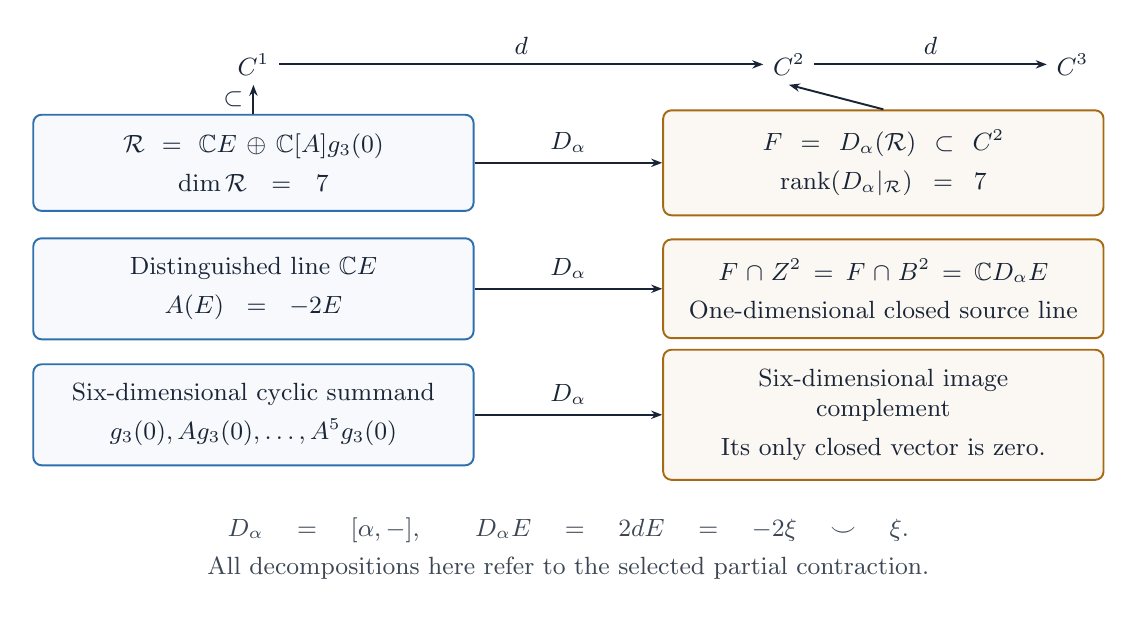
\begin{tikzpicture}
\node (c1) at (0,0) {$C^1$};
\node (c2) at (6.8,0) {$C^2$};
\node (c3) at (10.4,0) {$C^3$};
\draw[edge] (c1)--node[above]{$d$}(c2);
\draw[edge] (c2)--node[above]{$d$}(c3);
\node[box,text width=5.1cm] (r) at (0,-1.25)
 {$\R=\C E\oplus\C[A]g_3(0)$\\[3pt]$\dim\R=7$};
\node[goldbox,text width=5.1cm] (f) at (8,-1.25)
 {$F=D_\alpha(\R)\subset C^2$\\[3pt]$\operatorname{rank}(D_\alpha|_{\R})=7$};
\draw[edge] (r.north)--node[left]{$\subset$}(c1);
\draw[edge] (f.north)--(c2.south);
\draw[edge] (r)--node[above]{$D_\alpha$}(f);
\node[box,text width=5.1cm] (e) at (0,-2.85)
 {Distinguished line $\C E$\\[3pt]$A(E)=-2E$};
\node[goldbox,text width=5.1cm] (closed) at (8,-2.85)
 {$F\cap Z^2=F\cap B^2=\C D_\alpha E$\\[3pt]One-dimensional closed source line};
\draw[edge] (e)--node[above]{$D_\alpha$}(closed);
\node[box,text width=5.1cm] (cyc) at (0,-4.45)
 {Six-dimensional cyclic summand\\[3pt]
 $g_3(0),Ag_3(0),\ldots,A^5g_3(0)$};
\node[goldbox,text width=5.1cm] (non) at (8,-4.45)
 {Six-dimensional image\\complement\\[3pt]Its only closed vector is zero.};
\draw[edge] (cyc)--node[above]{$D_\alpha$}(non);
\node[note,text width=13.5cm] at (4,-6.15)
 {$D_\alpha=[\alpha,-],\qquad D_\alpha E=2dE=-2\xi\smile\xi$.\\[3pt]
 All decompositions here refer to the selected partial contraction.};
\end{tikzpicture}
\end{document}
